\documentclass[]{article}
\usepackage{amsmath}
\usepackage{verbatim}
\usepackage{geometry}
\usepackage{rotating}
\usepackage{subfigure}
\usepackage{hyperref}
\usepackage{graphicx}\geometry{
    paper=a4paper, % Change to letterpaper for US letter
    inner=1.5cm, % Inner margin
    outer=2.8cm, % Outer margin
    bindingoffset=.5cm, % Binding offset
    top=3.5cm, % Top margin
    bottom=1.5cm, % Bottom margin
    }
    \usepackage{empheq}
    \usepackage{xcolor}
    \newcommand{\boxedeq}[2]{\begin{empheq}[box={\fboxsep=6pt\fbox}]{align}\label{#1}#2\end{empheq}}
\title{Weekly report \textbf{09-10/16-10}}
\author{Marco Ghiani}
                        %  START THE DOCUMENTS
\begin{document}
\maketitle


\section{Targets of this week}
During this week my aims are: 
\begin{itemize}
   
   \item Run ten (differents Re$_\lambda$ number) Simulations and compute the PDFs of polymer length  
   \item Understanding of the algoritihms and data structuire  behind the computation of Histogram and PDF for the alignment of Eigenvector - spring    
   \item Improve Statistics and Probability knowledge of theory of Gaussian, mean value, standard deviations
\end{itemize}

\section {Simulations Computing PDFs for 30 Large Eddy T.O. Time}


%\begin{table}
% \centering
% \caption{Polymer molar mass = 3e7 g/mol}
%\label{table1}
%\begin{tabular}{ccccc}
%\hline
%\textbf{Quantities}& \textbf{54,74}& \textbf{56,72}& \textbf{57,76}& \textbf{58,78}\\ 
%\hline
%
%Pol Mol Mass&  3.0e+07 $g/mol$& 3.0e+07 $g/mol$& 3.0e+07 $g/mol$& 3.0e+07 $g/mol$\\ 
%
%$\tau_{LET}$ &     1.5694052$s$ &   1.6616610$s$ &   1.5059767$s$ &   1.3929481$s$\\ 
%$\Delta t$ &  0.0937500$cm$ &   0.0937500$cm$ &   0.0937500$cm$ &   0.0937500$cm$\\ 
%\hline
%$Re_\lambda$ &    71.6094889 &   69.3494276 &   71.7611996 &   77.6094351\\ 
%\\
%Deborah Number &     438.9014194 &   396.8298897 &   474.4528249 &   535.0524526\\ 
%Reynolds$_\lambda$ Number &    72.4968383 &   67.9388536 &   71.6177472 &   77.6937992\\ 
%Weissenberg Number &     101.9669240 &   93.9397317 &   110.5243930 &   119.4698450\\ 
%\end{tabular}
%\end{table}

\begin{table}[h]
 \centering
 \caption{Polymer molar mass = 3e7 g/mol}
\label{table1}
\begin{tabular}{cccccc}
\hline
\textbf{Quantities}       & \textbf{54,74}&   \textcolor{red}{\textbf{56,72}}&  \textbf{57,76}& \textbf{58,78}  & \textcolor{red}{\textbf{60,80}} \\ 
\hline


$\tau_{LET}$              &   1.5694052$s$ &   1.6616610$s$ &   1.5059767$s$ &   1.3929481$s$  &   1.3515364$s$  \\ 
$\Delta t$                &  $s$ & 1.3852E-3$s$  &  $s$ &   $s$ & 1.0474E-3$s$ \\ 
$ 20 \tau_{LET}$          &  $s$ &  33.23322$s$  &  $s$ &   $s$ & 27.030728$s$ \\
$ 30 \tau_{LET}$          &  $s$ &  49.84983$s$  &  $s$ &   $s$ & 40.546092$s$ \\
$N \Delta t (20LET)$              &      &   23991      &      &       &   25805      \\ 
$N \Delta t (30LET)$              &      &   35988      &      &       &   38711      \\ 
\hline
\\
De Num.                   &    438.9014194 &    396.8298897 &    474.4528249 &   535.0524526   &   569.9985655 \\ 
Re$_\lambda$ Num.         &     72.4968383 &     67.9388536 &     71.6177472 &   77.6937992    &   76.2821222 \\ 
We Num.                   &    101.9669240 &     93.9397317 &    110.5243930 &   119.4698450   &  128.9015288 \\ 
\end{tabular}
\end{table}

\begin{table}[h]
 \centering
 \caption{Polymer molar mass = 3e7 g/mol}
\label{table1}
\begin{tabular}{ccccccc}
\hline
\textbf{Quantities}&  \textbf{65,85}& \textcolor{red}{\textbf{75,95}}& \textbf{80,100}& \textcolor{red}{\textbf{85,106}}& \textbf{90,110}& \textcolor{red}{\textbf{95,120}}\\ 
\hline


$\tau_{LET}$ &     1.1841998$s$ &   0.9440772$s$ &   0.8491935$s$ &   0.7704134$s$ &   0.6949188$s$ &   0.5909659$s$\\ 
$\Delta t$       &      $s$ &   6.170E-4$s$ &   $s$ &    4.4040E-4$s$ &   $s$ & 2.9463E-4$s$\\ 
$ 20 \tau_{LET}$ &      $s$ &   18.88154$s$  &  $s$ &    15.408268$s$ &   $s$ & 11.819318$s$  \\
$ 30 \tau_{LET}$ &      $s$ &   28.32231$s$  &  $s$ &    23.112402$s$ &   $s$ & 17.728977$s$  \\
$N \Delta t (20LET)$              &     &  30602             &      & 34986           &     &40115    \\ 
$N \Delta t (30LET)$              &     &  45905             &      & 52480      &          &60175    \\ 

\hline
\\
De Num &     708.7409259 &   1065.6612932 &   1253.5101538 &   1533.7643768 &   1803.1746506 &   2410.2016353\\ 
Re$_\lambda$ Number &     81.3228611 &   94.0047870 &   96.3295600 &   103.1357506 &   111.7193443 &   117.7465437\\ 
We Number &      154.6182258 &  215.8799371 &   251.6512366 &   298.4699050 &   334.9042881 &   434.8471498\\ 
\end{tabular}
\end{table}






\section{Principal quantities plot}
\begin{figure}
   \centering
       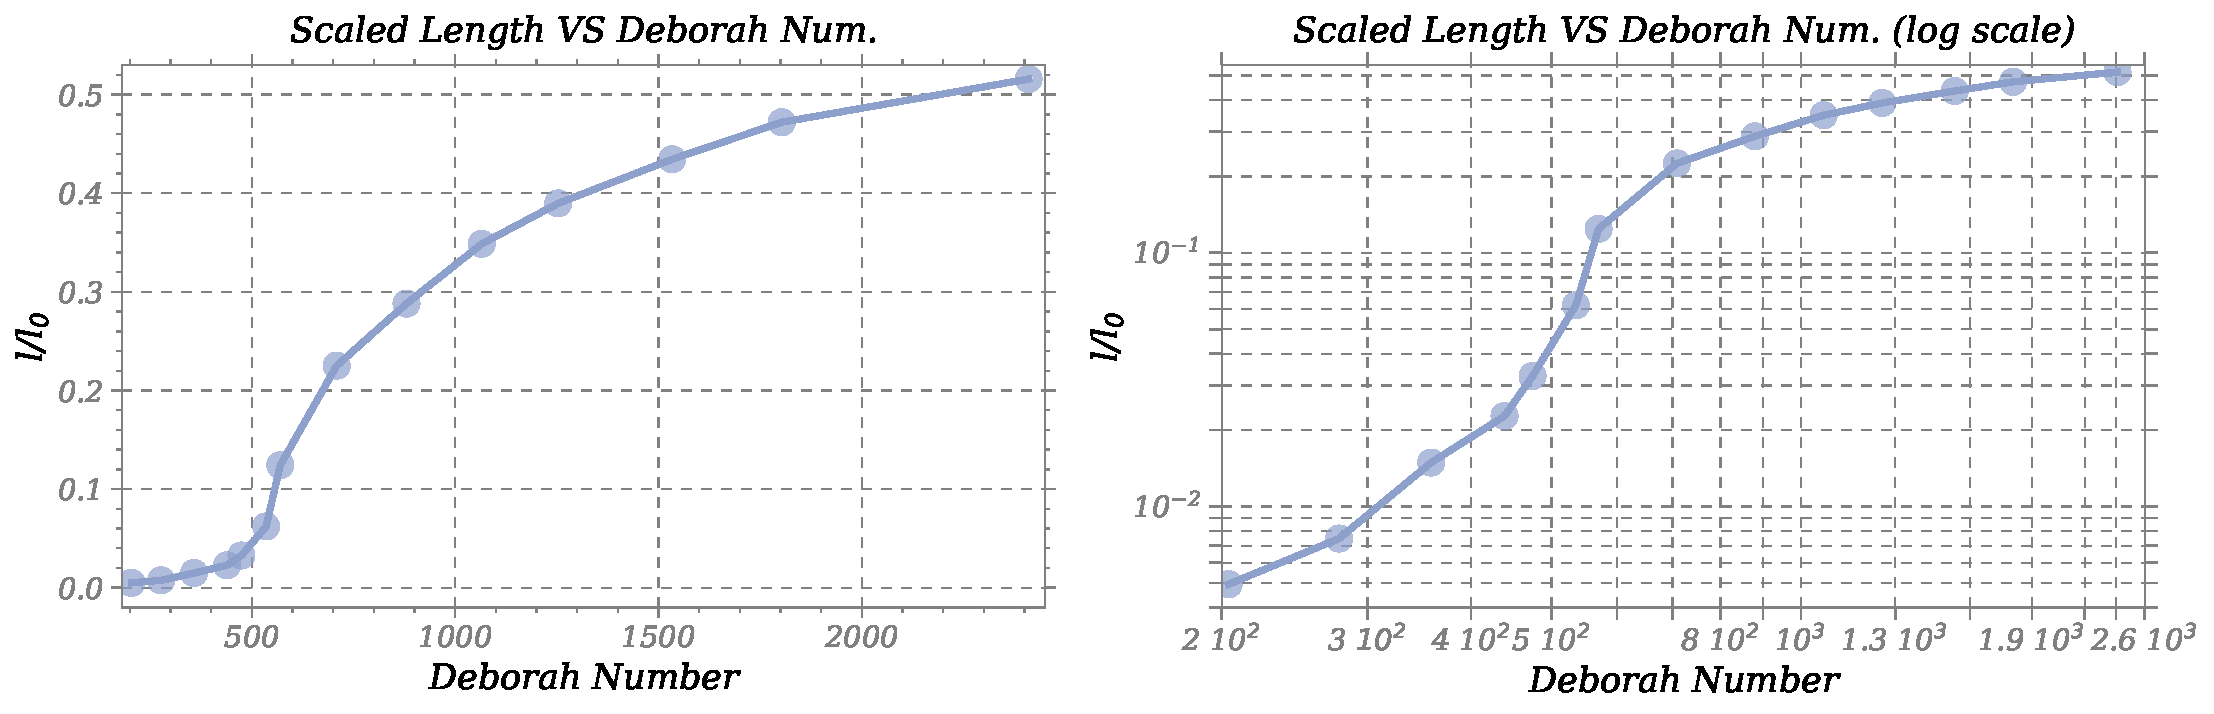
\includegraphics[width=1\textwidth]{DeborahNumber.pdf}
   \label{DeNum}
   \caption{Deborah number VS Pol. Scaled length}
\end{figure}
\begin{figure}
   \centering
       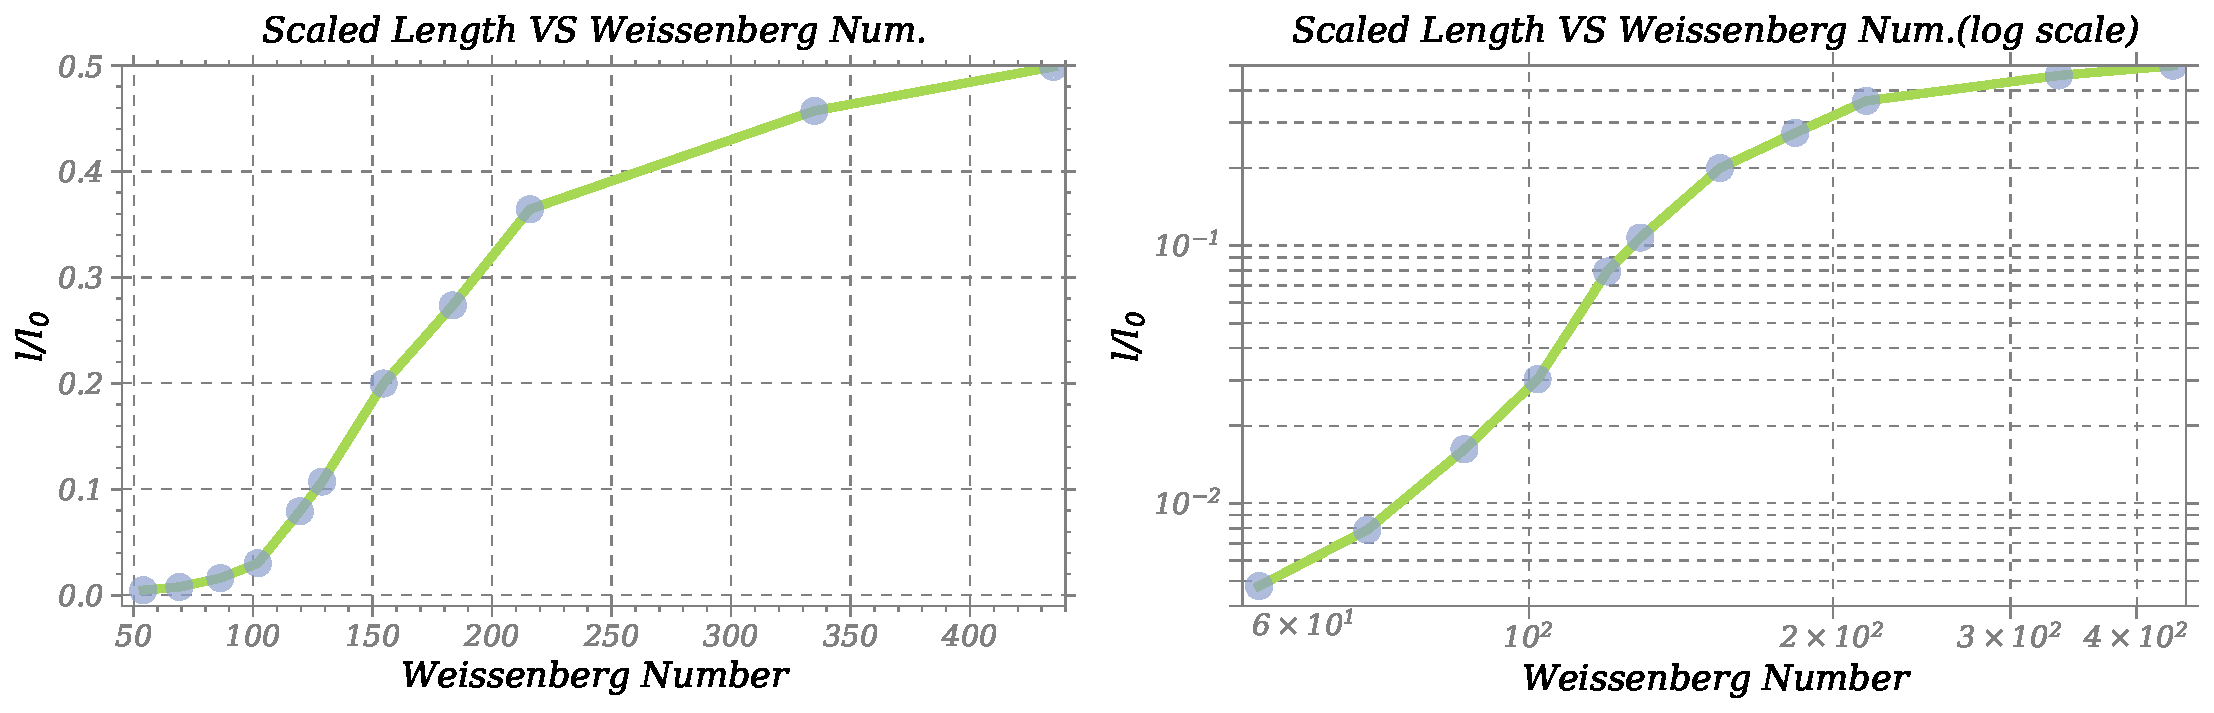
\includegraphics[width=1\textwidth]{WeissenbergNumber.pdf}
   \label{WeNum}
   \caption{Weissenberg number VS Pol. Scaled length}
\end{figure}
\begin{figure}
   \centering
       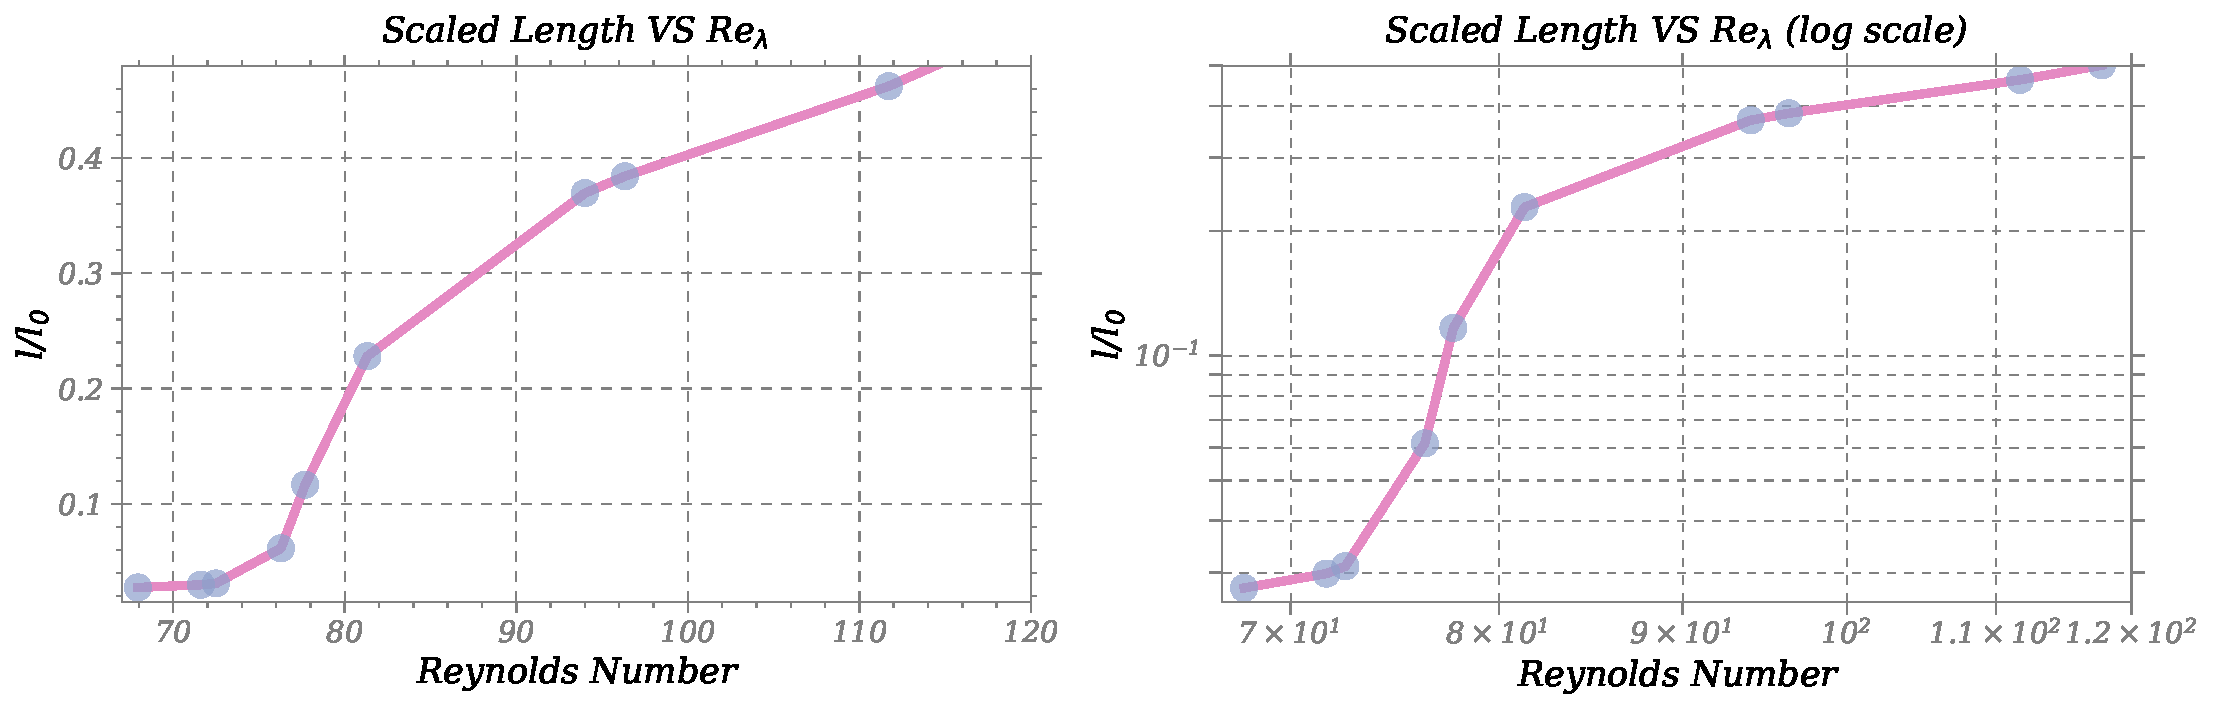
\includegraphics[width=1\textwidth]{ReynoldsTaylorNumber.pdf}
   \label{ReNum}
   \caption{Reynolds Taylor number VS Pol length}
\end{figure}
\begin{figure}[hb]
   \begin{center}
       \subfigure[][Deborah Number VS pol. scaled length]{
       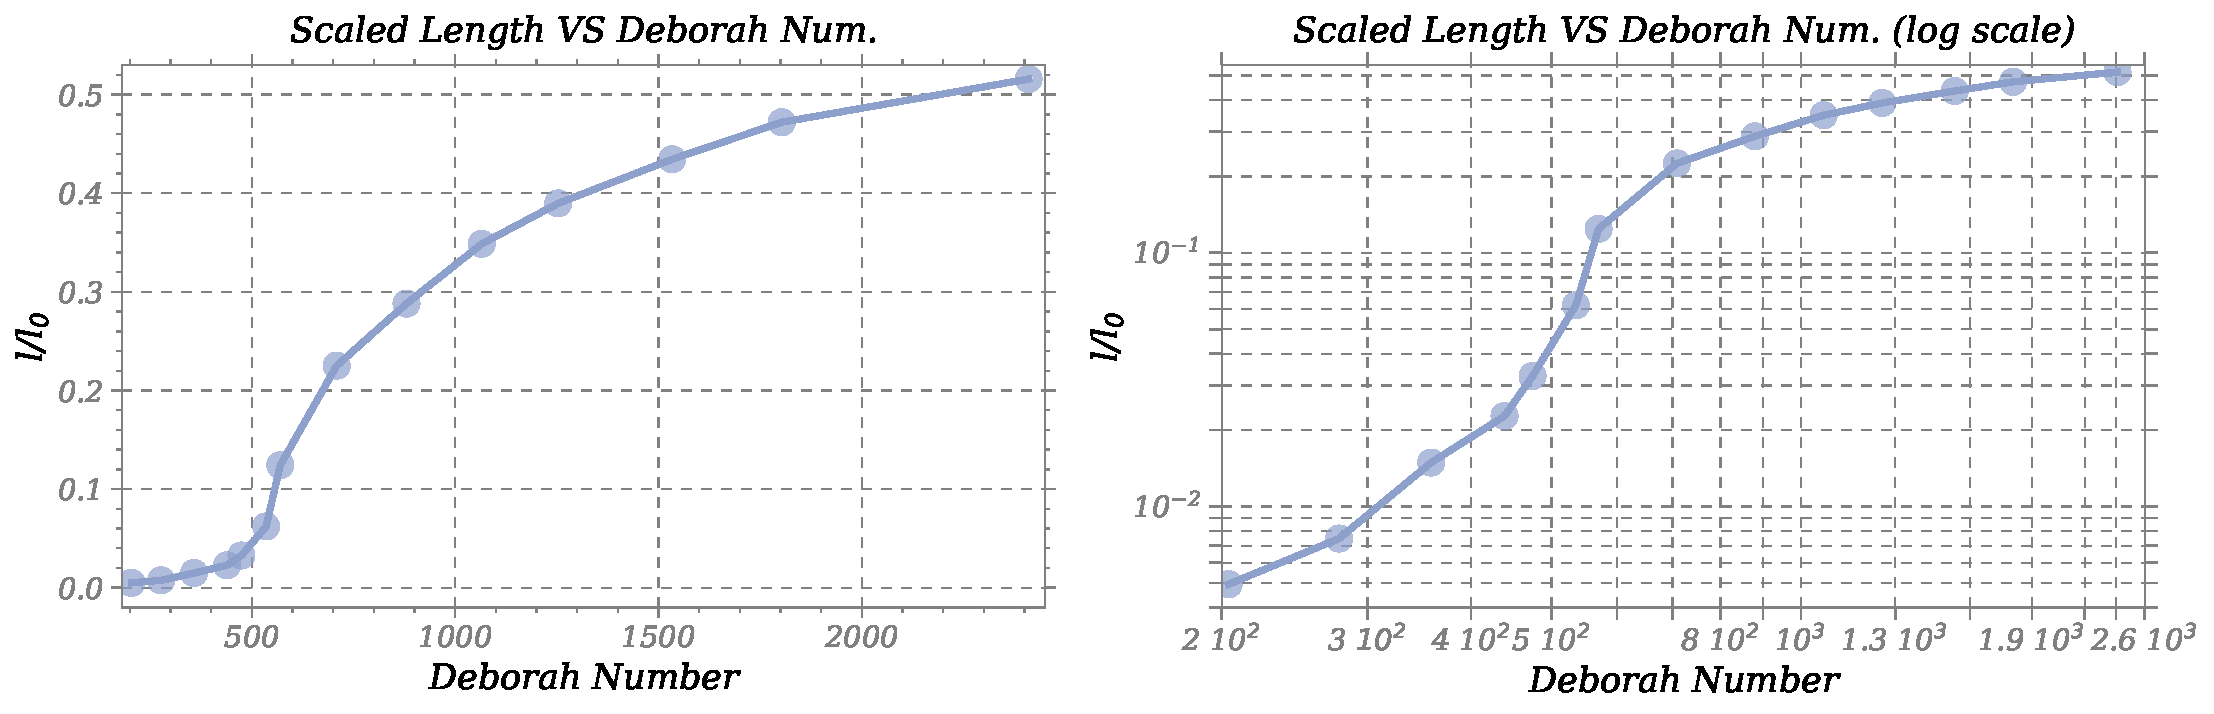
\includegraphics[width=1\textwidth]{DeborahNumber.pdf}
    \label{fig:1}
 }
        \subfigure[][Weissenberg number VS Pol. Scaled length]{
        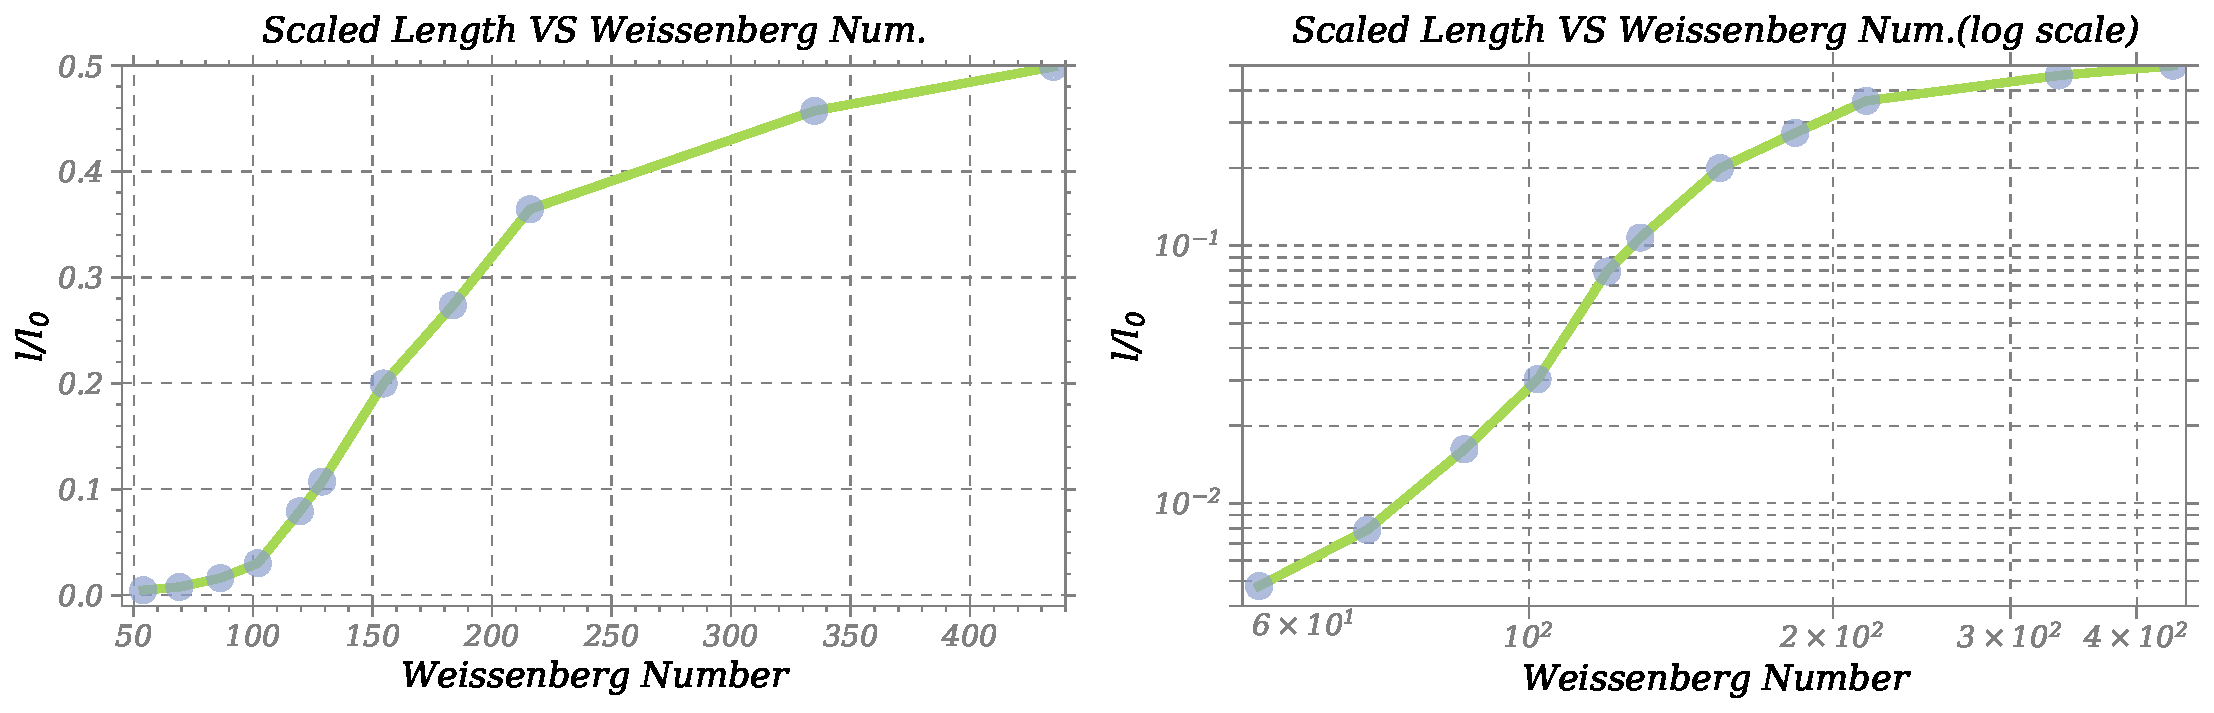
\includegraphics[width=1\textwidth]{WeissenbergNumber.pdf}
    \label{fig:2}
 }
        \subfigure[][Reynolds Taylor number VS Pol Scaled length]{
       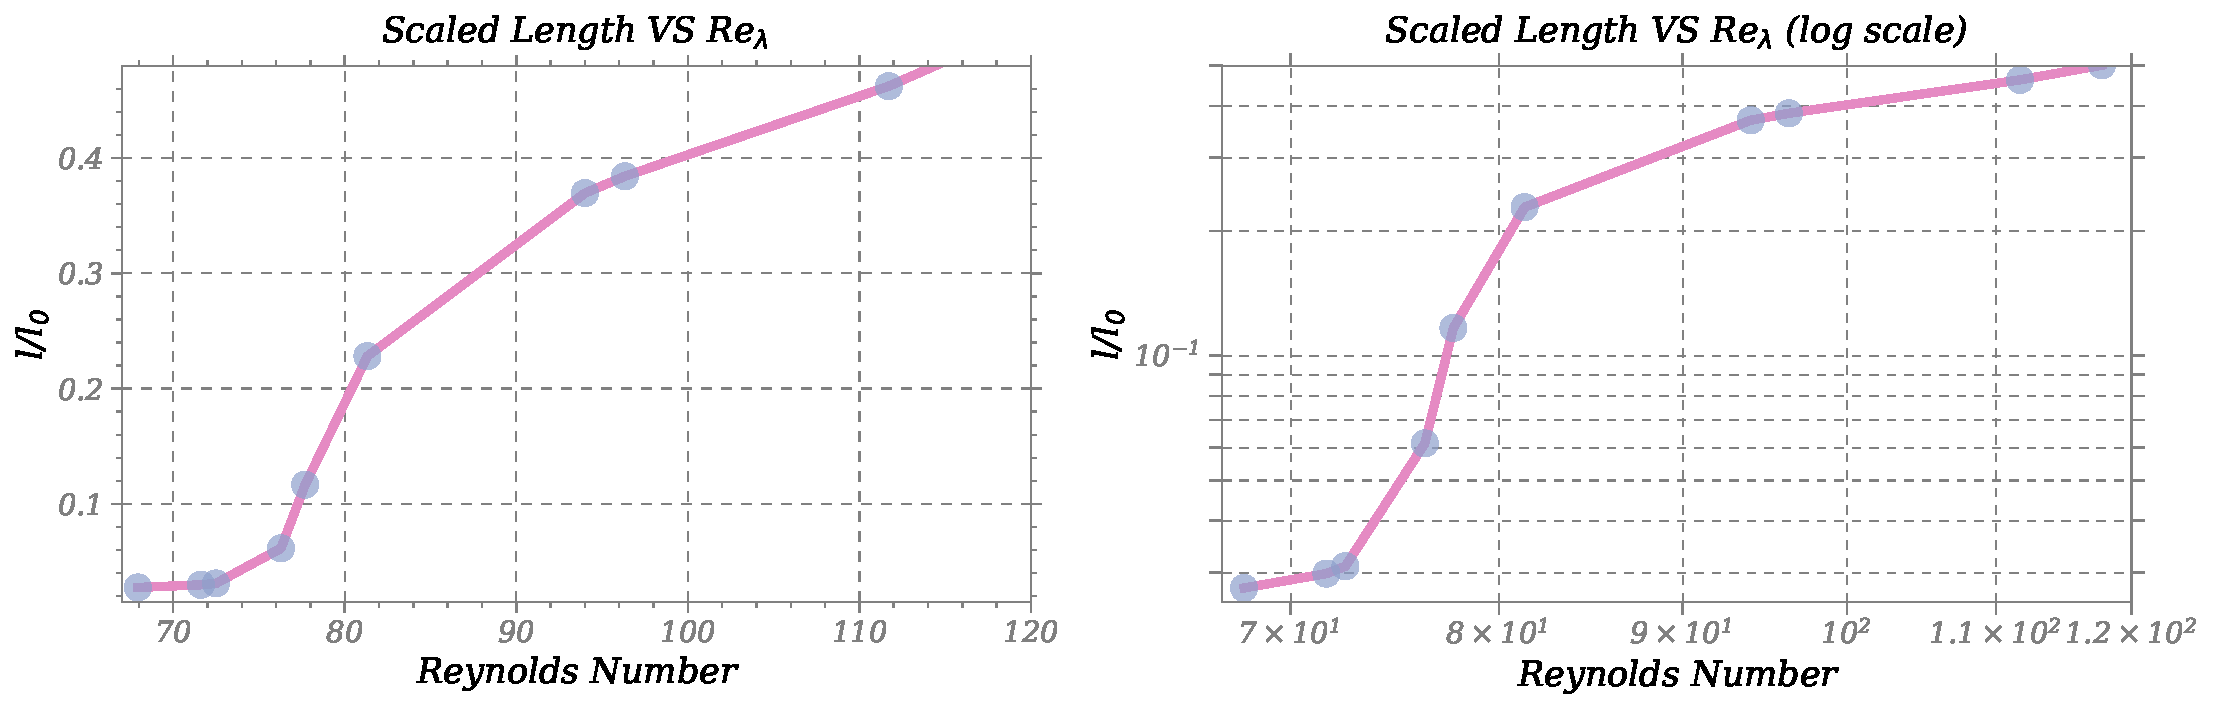
\includegraphics[width=1\textwidth]{ReynoldsTaylorNumber.pdf}
   \label{fig:3}
}
   \end{center}
   \caption{Principal polymer-flow quantities}
   \label{fig:quantities}
\end{figure}
\begin{figure}
   \centering
       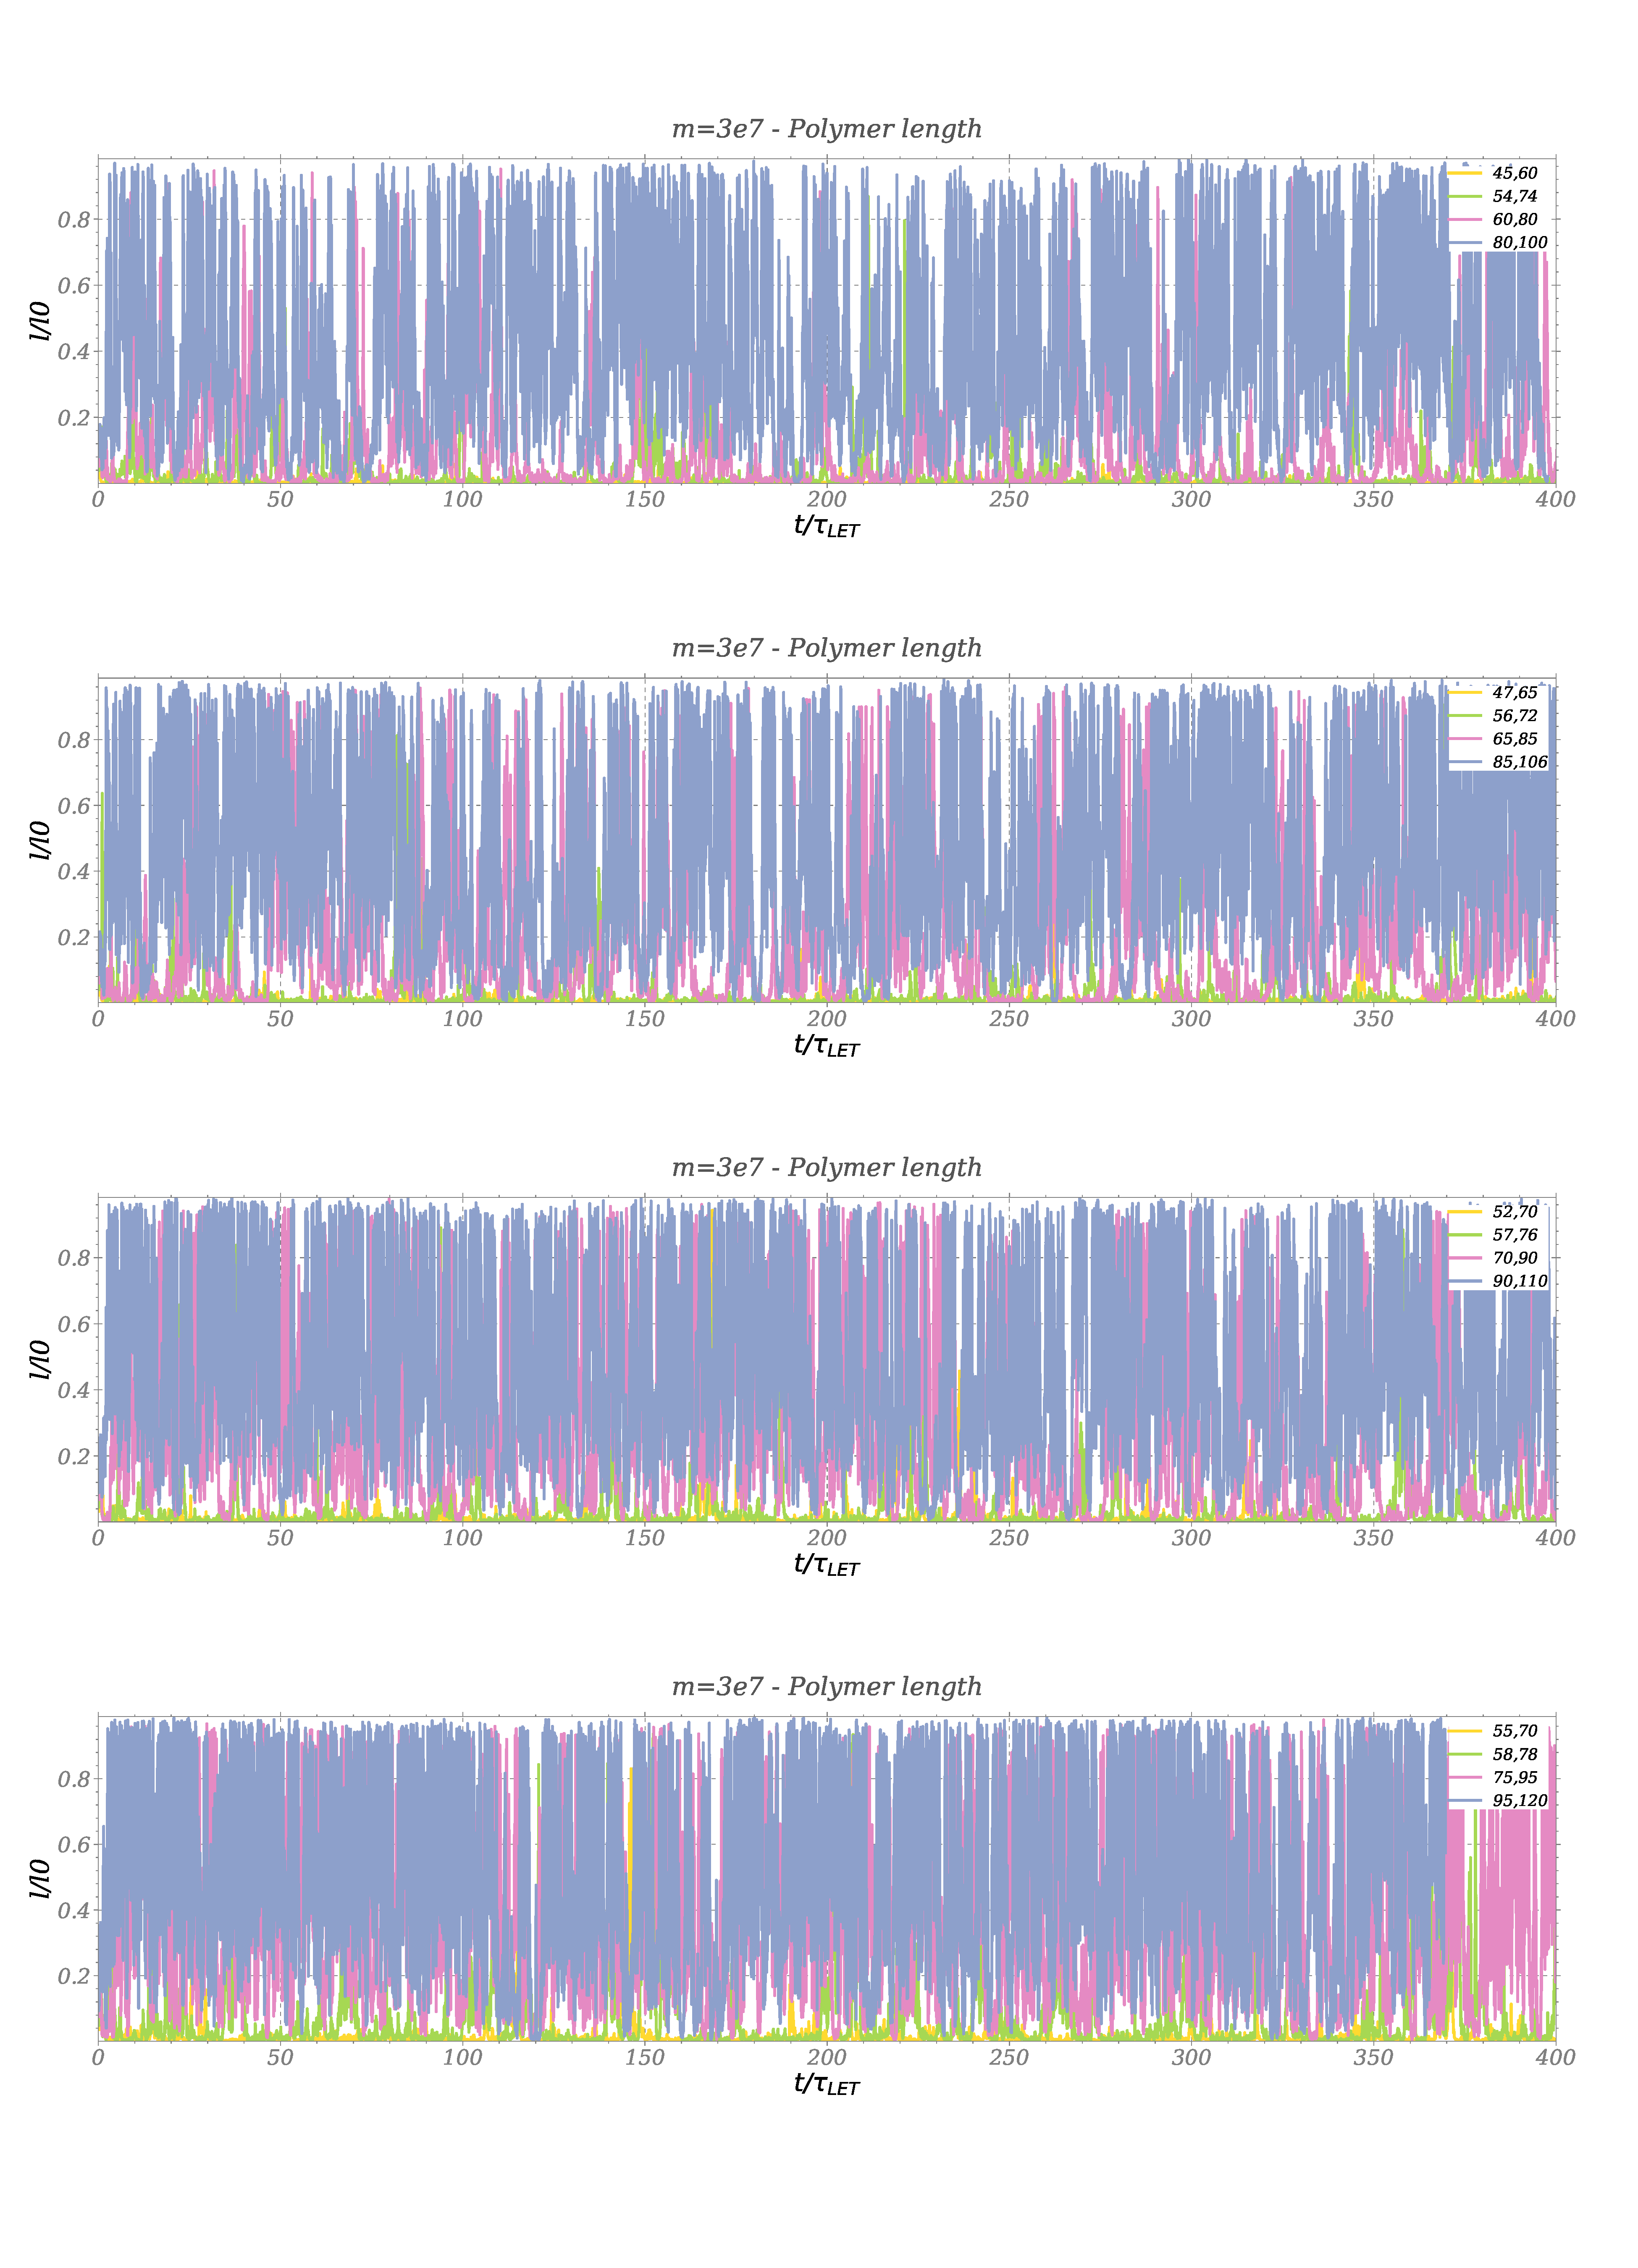
\includegraphics[width=1\textwidth]{timeVSlength.pdf}
   \label{ReNum}
   \caption{Time/$\tau_{LET}$  VS Pol chain Scaled length}
\end{figure}
\begin{figure}
   \centering
      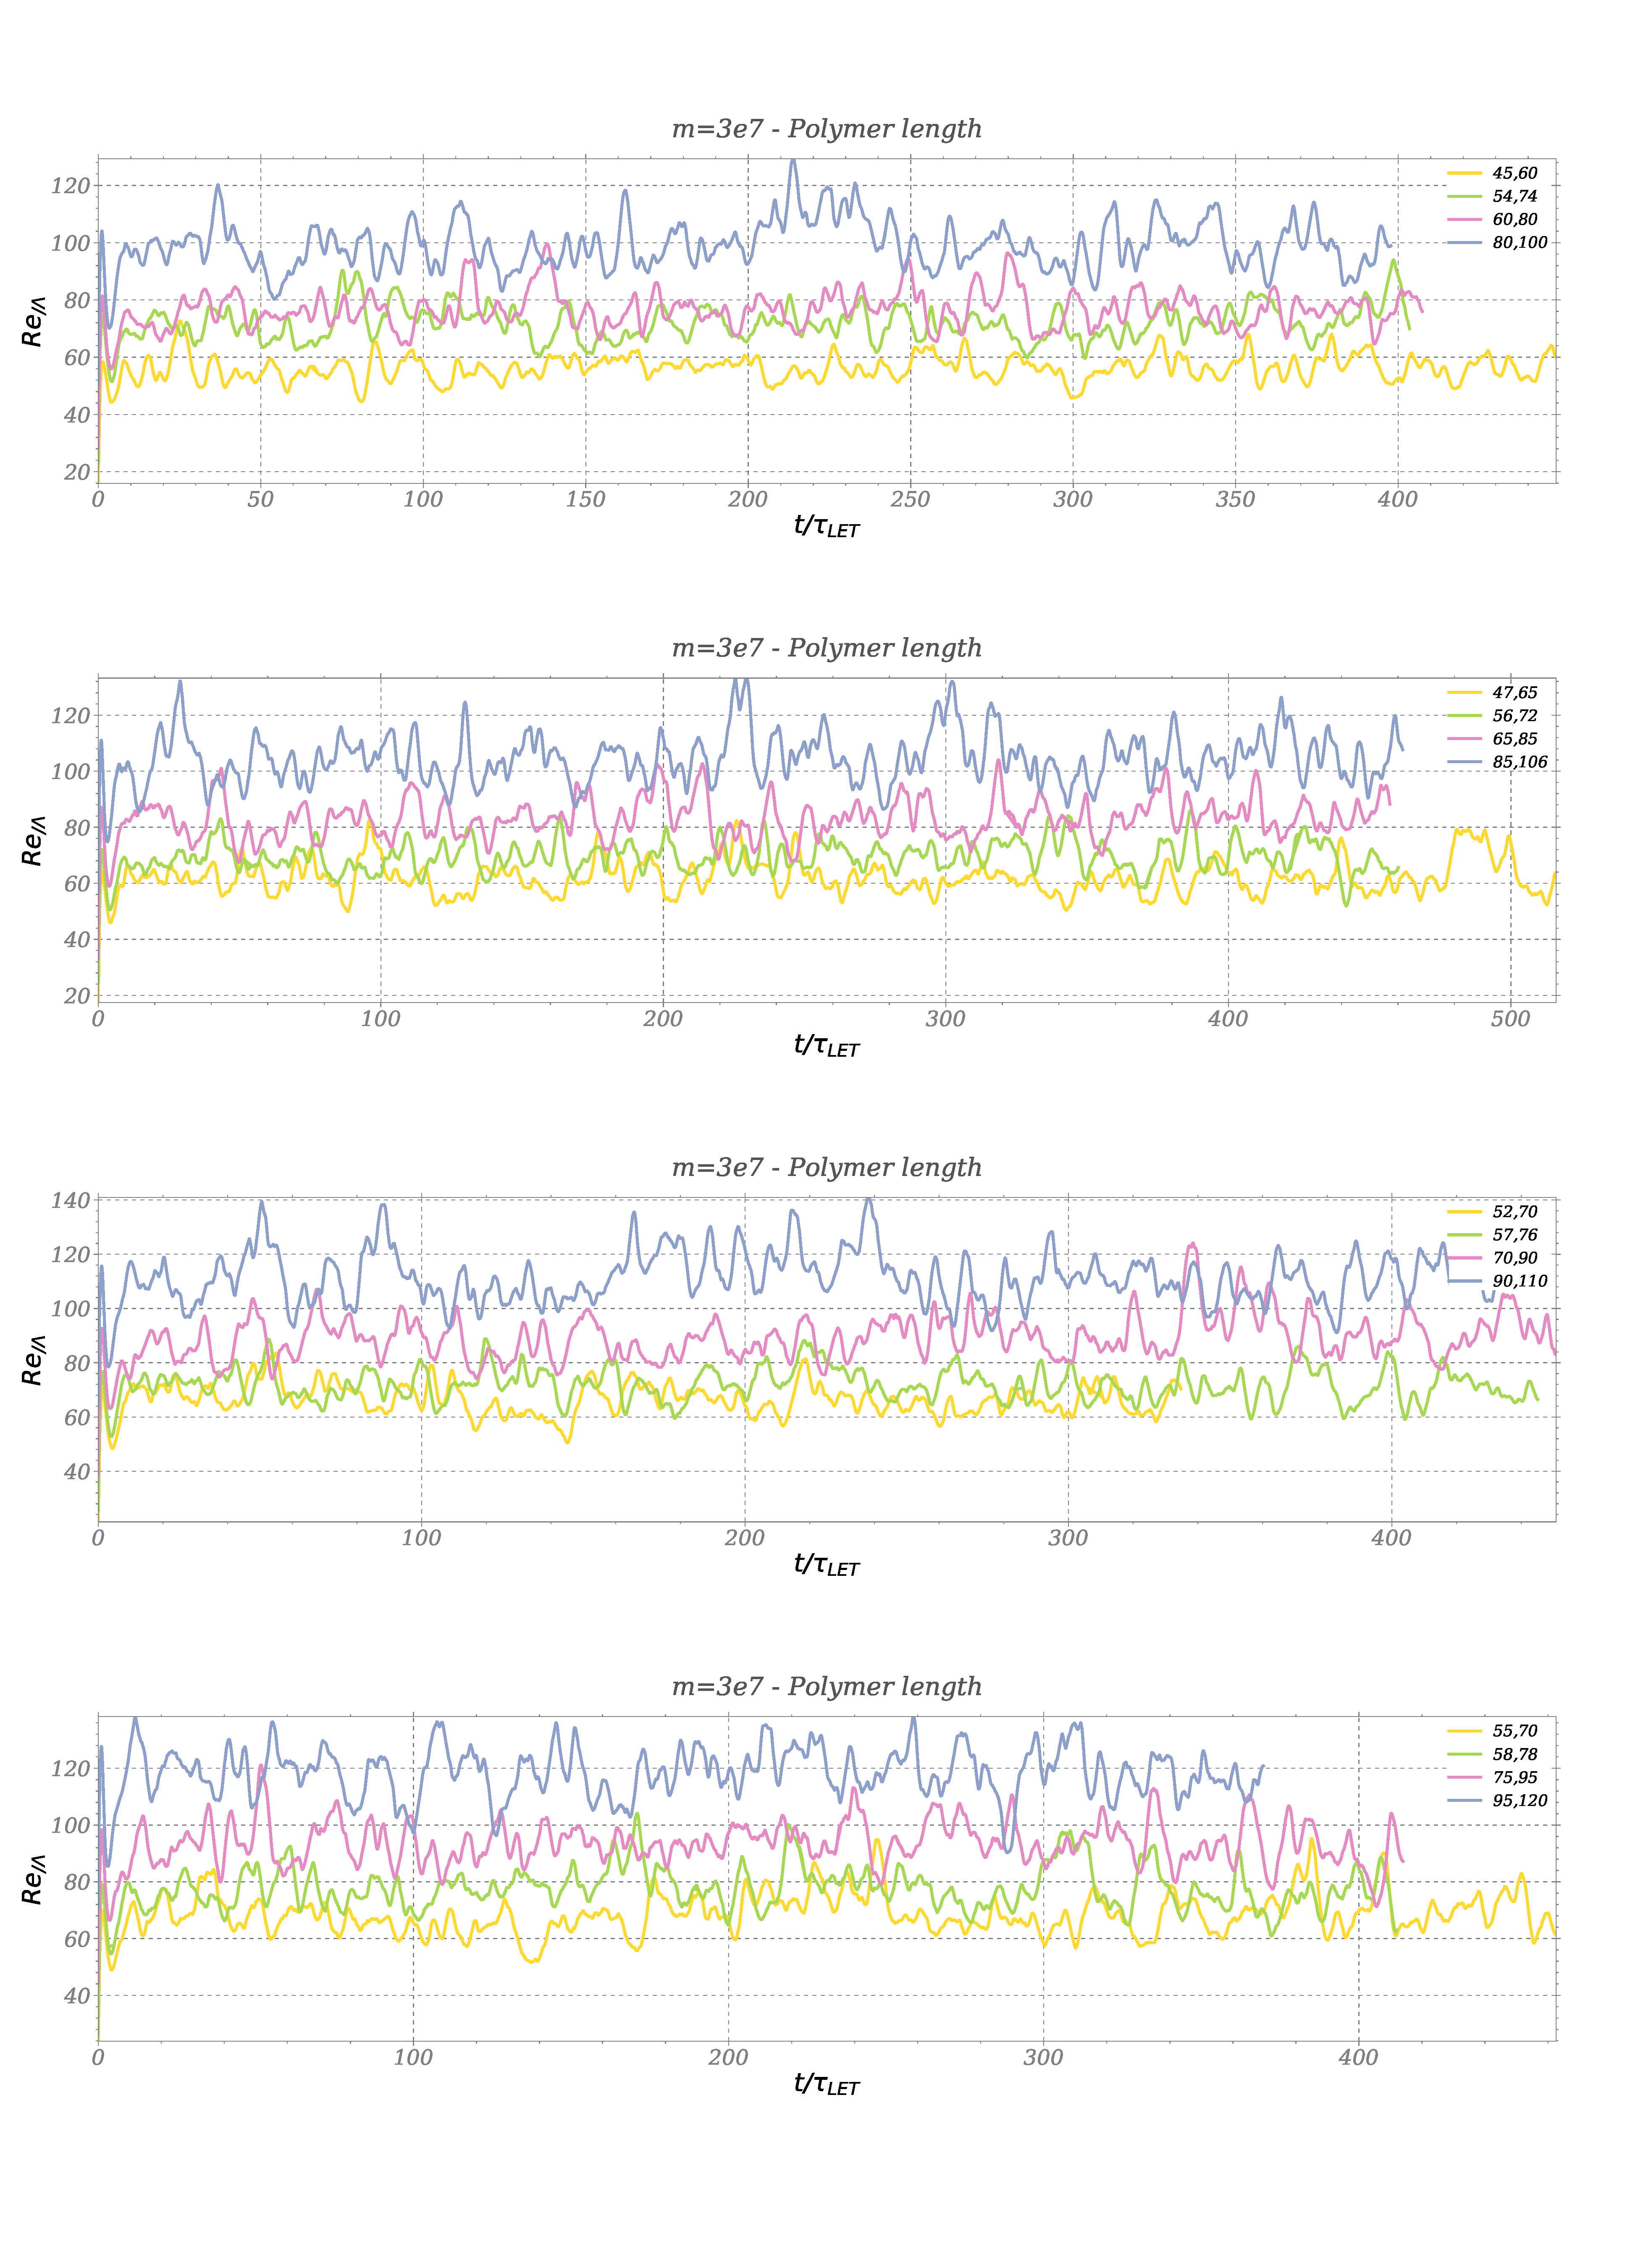
\includegraphics[width=1\textwidth]{timeVSreynolds.pdf}
   \label{ReNum}
   \caption{Time/$\tau_{LET}$  VS Reynolds Taylor Number}
\end{figure}
\section{Table of quantities}
\begin{sidewaystable}
 \centering
 \caption{Polymer molar mass = 3e7 g/mol}
\label{table1}
\begin{tabular}{ccccccccc}
\hline
\textbf{Quantities}& \textbf{45,60}& \textbf{47,65}& \textbf{52,70}& \textbf{55,70}& \textbf{54,74}& \textbf{56,72}& \textbf{57,76}& \textbf{58,78}\\ 
\hline

Pol Mol Mass& 3.0e+07 $g/mol$& 3.0e+07 $g/mol$& 3.0e+07 $g/mol$& 3.0e+07 $g/mol$& 3.0e+07 $g/mol$& 3.0e+07 $g/mol$& 3.0e+07 $g/mol$& 3.0e+07 $g/mol$\\ 

Kuhn monomer mm &  90.4977 &  90.4977 &  90.4977 &  90.4977 &  90.4977 &  90.4977 &  90.4977 &  90.4977\\ 
\hline

Zimm relax. t $\tau_0$ &   3.294868 &   3.294868 &   3.294868 &   3.294868 &   3.294868 &   3.294868 &   3.294868 &   3.294868\\ 
\hline

Pol.L Max \textcolor{red}{dimless} &   331500.0 [-] &   331500.0 [-] &   331500.0 [-] &   331500.0 [-] &   331500.0 [-] &   331500.0 [-] &   331500.0 [-] &   331500.0 [-]\\ 

Pol.L Max \textcolor{red}{dimens} &   2.443155E-02 $cm$ &   2.443155E-02 $cm$ &   2.443155E-02 $cm$ &   2.443155E-02 $cm$ &   2.443155E-02 $cm$ &   2.443155E-02 $cm$ &   2.443155E-02 $cm$ &   2.443155E-02 $cm$\\ 

Eq. chain sz  &  0.004474$l/l_{\text{Max}}$ &  0.004474$l/l_{\text{Max}}$ &  0.004474$l/l_{\text{Max}}$ &  0.004474$l/l_{\text{Max}}$ &  0.004474$l/l_{\text{Max}}$ &  0.004474$l/l_{\text{Max}}$ &  0.004474$l/l_{\text{Max}}$ &  0.004474$l/l_{\text{Max}}$\\ 
\hline
\\ 
$\lambda$ &   1.1590211$cm$ &   1.0814811$cm$ &   1.0032329$cm$ &   1.0172654$cm$ &   0.9576737$cm$ &   0.9820193$cm$ &   0.9209191$cm$ &   0.9209671$cm$\\ 
$\eta_{k}$ &   0.0789942$cm$ &   0.0698221$cm$ &   0.0624969$cm$ &   0.0624729$cm$ &   0.0574946$cm$ &   0.0599007$cm$ &   0.0552240$cm$ &   0.0531163$cm$\\ 
$\tau_\eta$ &   0.0609978$s$ &   0.0476551$s$ &   0.0381805$s$ &   0.0381512$s$ &   0.0323131$s$ &   0.0350743$s$ &   0.0298112$s$ &   0.0275791$s$\\ 
$\tau_{LET}$ &   2.4548560$s$ &   2.0491664$s$ &   1.7702274$s$ &   1.7444128$s$ &   1.5694052$s$ &   1.6616610$s$ &   1.5059767$s$ &   1.3929481$s$\\ 
$\Delta x$ &   0.0937500$cm$ &   0.0937500$cm$ &   0.0937500$cm$ &   0.0937500$cm$ &   0.0937500$cm$ &   0.0937500$cm$ &   0.0937500$cm$ &   0.0937500$cm$\\ 
$Re_\lambda$ &   55.3024803 &   61.9544777 &   66.5071021 &   68.4659170 &   71.6094889 &   69.3494276 &   71.7611996 &   77.6094351\\ 
\hline
\\
Deborah Number &   203.9586570 &   277.1527109 &   365.3290330 &   357.9898571 &   438.9014194 &   396.8298897 &   474.4528249 &   535.0524526\\ 
Reynolds$_\lambda$ Number &   55.6025678 &   62.7757427 &   67.7293609 &   65.6650012 &   72.4968383 &   67.9388536 &   71.6177472 &   77.6937992\\ 
Weissenberg Number &   54.0161340 &   69.1398309 &   86.2972186 &   86.3634367 &   101.9669240 &   93.9397317 &   110.5243930 &   119.4698450\\ 
\end{tabular}\end{sidewaystable}\begin{sidewaystable}
 \centering
 \caption{Polymer molar mass = 3e7 g/mol}
\label{table1}
\begin{tabular}{ccccccccc}
\hline
\textbf{Quantities}& \textbf{60,80}& \textbf{65,85}& \textbf{70,90}& \textbf{75,95}& \textbf{80,100}& \textbf{85,106}& \textbf{90,110}& \textbf{95,120}\\ 
\hline

Pol Mol Mass& 3.0e+07 $g/mol$& 3.0e+07 $g/mol$& 3.0e+07 $g/mol$& 3.0e+07 $g/mol$& 3.0e+07 $g/mol$& 3.0e+07 $g/mol$& 3.0e+07 $g/mol$& 3.0e+07 $g/mol$\\ 

Kuhn monomer mm &  90.4977 &  90.4977 &  90.4977 &  90.4977 &  90.4977 &  90.4977 &  90.4977 &  90.4977\\ 
\hline

Zimm relax. t $\tau_0$ &   3.294868 &   3.294868 &   3.294868 &   3.294868 &   3.294868 &   3.294868 &   3.294868 &   3.294868\\ 
\hline

Pol.L Max \textcolor{red}{dimless} &   331500.0 [-] &   331500.0 [-] &   331500.0 [-] &   331500.0 [-] &   331500.0 [-] &   331500.0 [-] &   331500.0 [-] &   331500.0 [-]\\ 

Pol.L Max \textcolor{red}{dimens} &   2.443155E-02 $cm$ &   2.443155E-02 $cm$ &   2.443155E-02 $cm$ &   2.443155E-02 $cm$ &   2.443155E-02 $cm$ &   2.443155E-02 $cm$ &   2.443155E-02 $cm$ &   2.443155E-02 $cm$\\ 

Eq. chain sz  &  0.004474$l/l_{\text{Max}}$ &  0.004474$l/l_{\text{Max}}$ &  0.004474$l/l_{\text{Max}}$ &  0.004474$l/l_{\text{Max}}$ &  0.004474$l/l_{\text{Max}}$ &  0.004474$l/l_{\text{Max}}$ &  0.004474$l/l_{\text{Max}}$ &  0.004474$l/l_{\text{Max}}$\\ 
\hline
\\ 
$\lambda$ &   0.8799067$cm$ &   0.8371844$cm$ &   0.7966835$cm$ &   0.7522937$cm$ &   0.7173550$cm$ &   0.6685970$cm$ &   0.6586933$cm$ &   0.5965867$cm$\\ 
$\eta_{k}$ &   0.0511361$cm$ &   0.0466903$cm$ &   0.0428607$cm$ &   0.0395140$cm$ &   0.0365980$cm$ &   0.0336052$cm$ &   0.0317246$cm$ &   0.0278412$cm$\\ 
$\tau_\eta$ &   0.0255611$s$ &   0.0213097$s$ &   0.0179574$s$ &   0.0152625$s$ &   0.0130930$s$ &   0.0110392$s$ &   0.0098382$s$ &   0.0075771$s$\\ 
$\tau_{LET}$ &   1.3515364$s$ &   1.1841998$s$ &   1.0486357$s$ &   0.9440772$s$ &   0.8491935$s$ &   0.7704134$s$ &   0.6949188$s$ &   0.5909659$s$\\ 
$\Delta x$ &   0.0937500$cm$ &   0.0937500$cm$ &   0.0937500$cm$ &   0.0937500$cm$ &   0.0937500$cm$ &   0.0937500$cm$ &   0.0937500$cm$ &   0.0937500$cm$\\ 
$Re_\lambda$ &   76.4004650 &   82.9653877 &   89.1723103 &   93.5042839 &   99.1296592 &   101.6910387 &   111.2697180 &   118.4440543\\ 
\hline
\\
Deborah Number &   569.9985655 &   708.7409259 &   880.1472967 &   1065.6612932 &   1253.5101538 &   1533.7643768 &   1803.1746506 &   2410.2016353\\ 
Reynolds$_\lambda$ Number &   76.2821222 &   81.3228611 &   88.4371104 &   94.0047870 &   96.3295600 &   103.1357506 &   111.7193443 &   117.7465437\\ 
Weissenberg Number &   128.9015288 &   154.6182258 &   183.4828856 &   215.8799371 &   251.6512366 &   298.4699050 &   334.9042881 &   434.8471498\\ 
\end{tabular}\end{sidewaystable}

\section{Numerical Algorithm for PDF}
\newpage
\subsection{Subroutine poly\_length}
\begin{verbatim}
 !--------------------------------------------------------
 !                                  poly_length
 !--------------------------------------------------------
 
 ! computes polymer length to obtain stochastics
 ! NOTE: ONLY beads are ordered along the chains;
 !       entanglements are NOT; the objects along
 !       a chain are NOT in increasing order
 
 subroutine poly_length(ppos,epos,ebflag,pstart,ppoints,polenpdf)
 
 use nrtype; use gencoms 
 use pol_lines_coms
 use chains
 
 implicit none
 
 real,dimension(0:nbeads-1,npdim),intent(in)::ppos
 real,dimension(1:netmax,npdim),intent(in)::epos
 integer,dimension(1:nbeads+2*netmax,npcon),intent(in)::ebflag
 integer,dimension(nchains),intent(in)::pstart
 integer,dimension(nchains),intent(in)::ppoints
 real,dimension(lenbins),intent(inout)::polenpdf
 real,dimension(npdim)::pnext,plast,diff,pcur
 real::c_len,elbalen,magdiff
 integer::i,ic,ib,nbeg,nend,next,cur
 
 do_chains:do ic=1,nchains
 
   c_len=0.0                !zero chain length
 
   nbeg=pstart(ic)+1               !from ppos to ebflag convention for beads
   nend=pstart(ic)+ppoints(ic)-1   !excludes chain ends
 
   beads:do ib=nbeg,nend           !loop all beads in the chain
 
     elbalen=0.0                   !zero the elastic band length
     cur=ib
     pcur(:)=ppos(cur-1,:)
 
     indef:do
       next=ebflag(cur,1)
       if(polbou == 'perbou')then
         call ebp_unwrap(cur,ebflag,ppos,epos,pnext,plast)
       else
         call find_opos(next,ppos,epos,pnext(1),pnext(2),pnext(3))
       endif
       diff=pnext-pcur
       magdiff=sqrt(sum(diff(1:npdim)*diff(1:npdim)))
       elbalen=elbalen+magdiff
       if(next <= nbeads) exit indef           !reached the other bead-end of this spring
       cur=next                                !the next eb is an entanglement
       pcur(:)=epos(int((cur-nbeads+1)/2),:)
     enddo indef
 
     c_len=c_len+elbalen                       !add to chain length
 
   enddo beads
 
                              !add the new chain length information to the histogram
 
   c_len=c_len/lchaimx        !normalize to have (0,1) values
   loop:do i=1,lenbins
     if(c_len > real(i-1)/real(lenbins) .and. c_len <= real(i)/real(lenbins))then
       polenpdf(i)=polenpdf(i)+1
       exit loop
     endif
   enddo loop
 
enddo do_chains
 
end subroutine poly_length

\end{verbatim}

\subsection{Subroutine poly\_length\_stoch}
\begin{verbatim}
!--------------------------------------------------------------------
!                                              poly_length_stoch
!--------------------------------------------------------------------

 !pdf for polymer chain lengths
 
 
 subroutine poly_length_stoch(polenpdf)
 
 use nrtype; use gencoms
 use pol_lines_coms
 
 implicit none
 
 real,dimension(lenbins),intent(in)::polenpdf
 real::norm,vvalue,pvalue,mlen,sdlen,sfac,dfac
 integer::i
 
 norm=0.
 do i=1,lenbins
   norm=norm+polenpdf(i)/real(lenbins)  !integrate histogram
 enddo
 
         !unit 62 is polenpdf.dat
 
 rewind(62)
 write(62,"('  TIME T=',f18.10)") time*unitt
 mlen=0.0
 do i=1,lenbins
   vvalue=(0.5*(real(i)+real(i-1)))/real(lenbins)
   pvalue=polenpdf(i)/norm
   write(62,'(2(1x,e34.26))')vvalue,pvalue       !normalized histogram--->pdf
   mlen=mlen+pvalue*vvalue/real(lenbins)         !E(x)
 enddo
 
        !unit 63 is mpolen.dat
 
 write(63,'(2(1x,e34.26))')time*unitt,mlen       !mean polymer length
 
        !compute standard deviation to fit Gaussians
 
 sdlen=0.
 do i=1,lenbins
   vvalue=(0.5*(real(i)+real(i-1)))/real(lenbins)
   pvalue=polenpdf(i)/norm
   sdlen=sdlen+pvalue*((vvalue-mlen)**2.)/real(lenbins)    !E((x-E[x])^2)
 enddo
 sdlen=sqrt(sdlen)             !standard deviation sigma
 
        !unit 64 is polengau.dat
 
 rewind(64)
 write(64,"('  TIME T=',f18.10)") time*unitt
 sfac=1./(sqrt(twopi)*sdlen)
 dfac=1./(2.*sdlen**2.)
 do i=1,lenbins
   vvalue=(0.5*(real(i)+real(i-1)))/real(lenbins)
   pvalue=sfac*exp(-dfac*(vvalue-mlen)**2.)
   write(64,'(2(1x,e34.26))')vvalue,pvalue          !corresponding Gaussian
 enddo
 
 end subroutine  poly_length_stoch


\end{verbatim}

\section{Call points of this routine}

Using the \verb|grep| tools I had check al the points in which this 2 subroutine are called.  
\begin{verbatim}
grep -F "call poly_length_stoch" *.f90
polout.f90:  if(ipolestoch == 1)call poly_length_stoch(polenpdf)
\end{verbatim}
\begin{verbatim}
grep -F "call poly_length" *.f90
polout.f90:if(ipolestoch == 1)call poly_length(ppos,epos,ebflag,pstart,ppoints,polenpdf)
\end{verbatim}
\end{document}
